\documentclass{standalone}
\usepackage{tikz}
\begin{document}
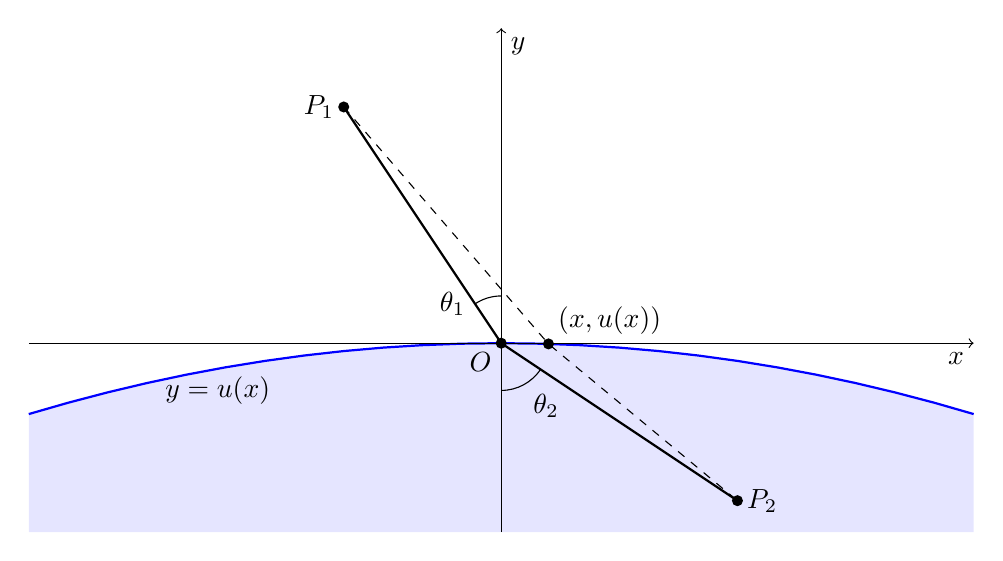
\begin{tikzpicture}[scale=2]
    % Surface (parabolic for illustration)
    \fill[blue!10] (-3,-1.2) -- (3,-1.2) -- plot[domain=3:-3] (\x, {-0.05*\x*\x}) -- cycle;
    \draw[thick, blue, domain=-3:3] plot (\x, {-0.05*\x*\x});
    \node at (-1.8,-0.3) { \( y = u(x) \) };

    % Axes
    \draw[->] (-3,0) -- (3,0) node[below left]{$x$};
    \draw[->] (0,-1.2) -- (0,2) node[below right]{$y$};
    
    
    % Point O
    \fill (0,0) circle (1pt) node[below left]{$O$};
    
    % Incident ray
    \draw[thick] (-1,1.5) -- (0,0);
    \fill (-1,1.5) circle (1pt) node[left]{$P_1$};
    
    % Refracted ray
    \draw[thick] (0,0) -- (1.5,-1);
    \fill (1.5,-1) circle (1pt) node[right]{$P_2$};
    
    % Variation ray
    \draw[dashed] (-1,1.5) -- (0.3,{-0.05*0.3*0.3}) -- (1.5,-1);
    \fill (0.3,{-0.05*0.3*0.3}) circle (1pt) node[above right]{$(x,u(x))$};

    % Angle θ1
    \draw (0,0.3) arc (90:123.69:0.3) node[left]{$\theta_1$};
    
    % Angle θ2
    \draw (0,-0.3) arc (-90:-33.69:0.3) node[midway, below right]{$\theta_2$};
    
\end{tikzpicture}
\end{document}